\section{Application architecture}

In this part I will first focus on the architecture chosen to make the link between the graphical interface and the business logic of the application, then I will describe the architecture adopted to implement the different exercises within the application.

The class diagram of the project architecture with the different classes that were used is available in appendix \ref{appendix:class}.

\subsection{GUI and business logic}
The GUI of the application and the business logic must of course be separate. In addition, the business logic must be independent of the GUI. This allows for example to deploy a web and mobile application with the same business logic, and by simply defining 2 different interfaces for web and mobile.

The application architecture is a crucial choice in application development. The modification of the data in the business logic must be reflected in the GUI. A graphic component in Flutter is called \textit{widget} (button, text, layout, etc.). Mobile programming is asynchronous and reactive, data can be modified after a network call, by an external user or by another device for example; widgets must react to these changes.

I chose to add a layer of providers between the GUI level and the business logic level. These providers provide the necessary data to the GUI through \textit{stream} (equivalent to \textit{observable} in \textit{ReactiveX}). Here, a stream can be seen as a unidirectional pipe, the provider inserts elements into this pipe, and the graphic part has access to the second end of the pipe to access the element in the pipe. Each new element inserted in the \textit{stream} replaces the eventual old element.

\begin{figure}[H]
  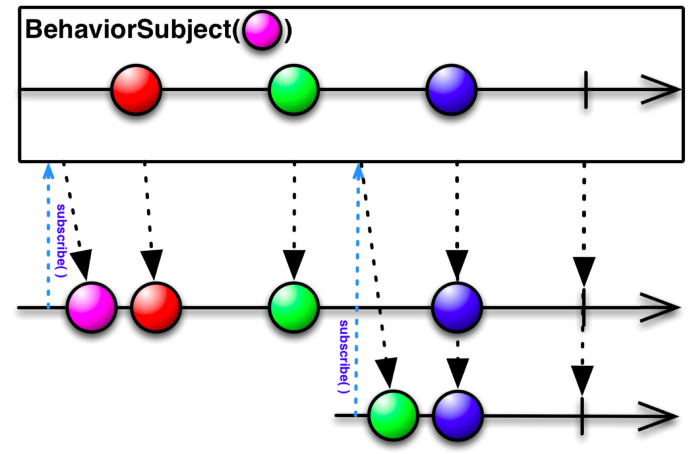
\includegraphics[width=.7\linewidth]{content/imgs/stream.png}
  \caption{\textit{Behaviour subject}}
  \label{fig:stream}
\end{figure}

There is the widget \textit{StreamBuilder} which allows you to listen to the output of a \textit{stream}. Each new element inserted in the stream has the effect of rebuild the descendants of this widget: children of this widget will be rebuilt and redrawn on the screen. For example, if the text field of the widget tree in figure \ref{fig:stream_ex1} depends on a data of the business logic that is likely to change over time and is therefore available via a \textit{stream},  \textit{StreamBuilder} widget has to be add as the parent to this text widget. The \textit{StreamBuilder} widget will have access to the end of the pipe containing the data to be displayed. This widget and therefore its descendants (and therefore the text field) will be automatically rebuilt each time the stream content changes (i.e. the provider inserts a new data into the pipe).

This architecture allows to rebuild only parts of the GUI that \textbf{need} to be rebuilt following the modification or addition of a data, which is done on the business logic side of the application. It is a much more powerful architecture than a basic solution that would consist in rebuilding the entire widget tree from the root of the page displayed each time it is changed.

\begin{figure}[H]
  \centering
  \begin{subfigure}{.5\textwidth}
    \centering
    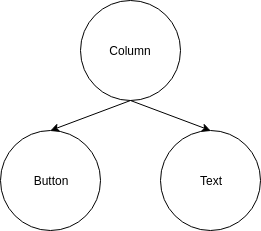
\includegraphics[width=.8\linewidth]{content/imgs/ex1.png}
    \caption{Widgets tree}
    \label{fig:stream_ex1}
  \end{subfigure}%
  \begin{subfigure}{.5\textwidth}
    \centering
    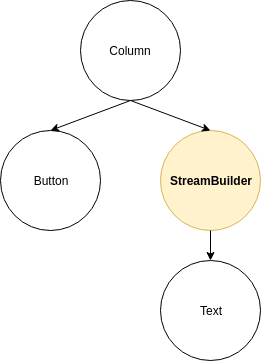
\includegraphics[width=.8\linewidth]{content/imgs/ex2.png}
    \caption{Same tree with a \textit{StreamBuilder}}
  \end{subfigure}
  \caption{\textit{StreamBuilder} example}
\end{figure}

\subsection{Exercise architecture}

One aspect of the application that was interesting to design was the exercise structure. The exercises are different but still share many common points, so it was necessary to find an architecture that would allow different exercises to be implemented quickly without re-developing the entire exercise base each time.

\begin{figure}[H]
  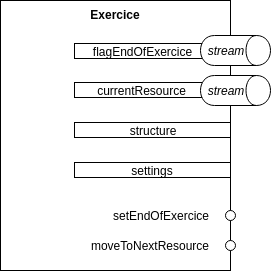
\includegraphics[width=150px]{content/imgs/exercice.png}
  \caption{Exercice structure}
  \label{fig:exercice}
\end{figure}

The architecture chose is as follows: an exercise simply has the following attributes:

\begin{itemize}
  \item Une \textbf{strucutre} : the list of elements that the exercise is made up. Several elements can be used by an exercise, for example: a voice recorder, a word, sentence or text display, a metronome, etc.;
  \item Des \textbf{settings} : the settings of the exercise (chose by the user or directly imposed by the exercise). These settings are identified by an ID and associated with a value (boolean, integer, etc.);
  \item La \textbf{current resource} : the resource currently used by the exercise (word, sentence, text);
  \item A \textbf{flag} to signal the end of the exercise.
\end{itemize}

\textit{Note: to make it simple, I omitted some information such as creation date, title, etc).}

\paragraph{Structure}
As seen above, the structure of an exercise is made up of several elements (concretely these elements are the values of an enumerated type). On the graphical side, there is a converter of these values into a graphical widget. For example, the element \textit{metronome} will be associated with a widget that displays a metronome with a visual signal and a sound signal at a regular tempo. These graphical objects have access to the attributes and to certain methods of the exercise. For example, the widget to display a resource (word, sentence, text), has access to the current resource of the exercise and can call the function \texttt{moveToNextResource} to change the current resource. These widgets can also access the exercise settings.

\begin{figure}[H]
  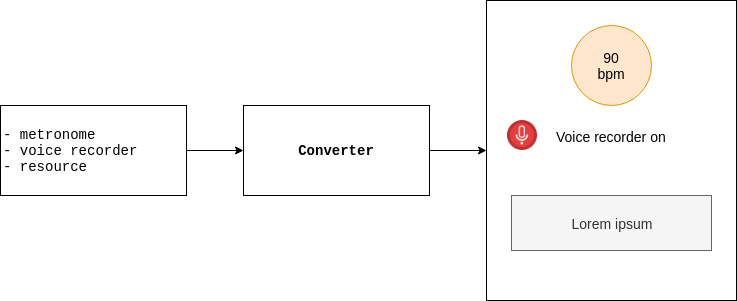
\includegraphics[width=0.8\linewidth]{content/imgs/struc.png}
  \caption{From the structure to the interface}
  \label{fig:struc}
\end{figure}

\paragraph{Settings}
Each exercise can define its list of settings. These settings are intended for use by the \textit{widgets} associated with the elements of the exercise structure. For example, the metronome exercise can define a setting \texttt{metronome\_bpm} that will allow the widget displaying the metronome to set the tempo value according to this setting. As with the elements of the exercise structure, there is a converter of the settings into a graphical widget to modify these settings.

\begin{figure}[H]
  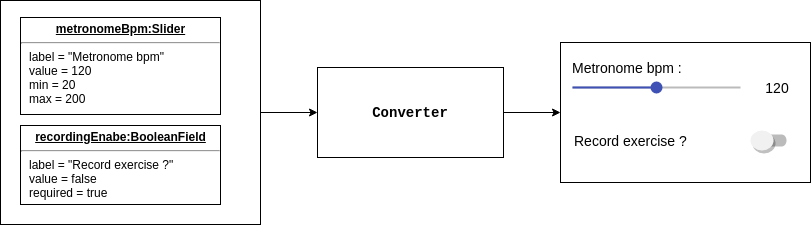
\includegraphics[width=0.8\linewidth]{content/imgs/settings.png}
  \caption{Visual generation of exercise settings}
  \label{fig:settings}
\end{figure}

This architecture makes it easy and fast to build a wide range of exercises. To structure a new exercise, it is only necessary to use the existing collection if all the elements necessary for the creation of the exercise are available. In this case, it is just a necessary to develop the missing element.






% eof
